\documentclass[12pt]{article}
\usepackage[T1]{fontenc}
\usepackage[utf8]{inputenc}
\usepackage[english]{babel}
\usepackage{amsthm}
\usepackage{amsmath}
\usepackage{amssymb}
\usepackage{fullpage}
\usepackage{authblk}
\usepackage{hyperref}
\usepackage{graphicx}
\usepackage{color}



%\def\emph{#1}\textbf{#1}
\makeatletter
\numberwithin{equation}{section} %% Comment out for sequentially-numbered
\numberwithin{figure}{section} %% Comment out for sequentially-numbered
\def\proof{\noindent{\bf Proof: }}
\def\qed{ \hskip 20pt{\vrule height7pt width6pt depth0pt}\hfil}

\def\area{{\text{Area}}} %% This is probably the wrong way to do it. Breña: fix it.
\def\cA{{\mathcal{A}}}
\def\cB{{\mathcal{B}}}
\def\cF{{\mathcal{F}}}
\def\cC{{\mathcal{C}}}
\def\cD{{\mathcal{D}}}
\def\cM{{\mathcal{M}}}
\def\cO{{\mathcal{O}}}
\def\cI{{\mathcal{I}}}
\def\cV{{\mathcal{V}}}
\def\cU{{\mathcal{U}}}
\def\cT{{\mathcal{T}}}
\def\cP{{\mathcal{P}}}
\def\cS{{\mathcal{S}}}
\def\cX{{\mathcal{X}}}
\def\cY{{\mathcal{Y}}}

\def\NN{{\mathbb{N}}}
\def\RR{{\mathbb{R}}}
\def\ZZ{{\mathbb{Z}}}

\theoremstyle{definition}
\newtheorem{theorem}{Theorem}[section]
\newtheorem{lemma}[theorem]{Lemma}
\newtheorem{example}[theorem]{Example}
\newtheorem{proposition}[theorem]{Proposition}
\newtheorem{corollary}[theorem]{Corollary}
\newtheorem{conjecture}[theorem]{Conjecture}
\newtheorem{definition}[theorem]{Definition}
\newtheorem{remark}[theorem]{Remark}
\newtheorem{observation}[theorem]{Observation}
\newtheorem{problem}[theorem]{Problem}
% \makeatother

\definecolor{MyBlue}{RGB}{0,0,255}
\definecolor{MyRed}{RGB}{255,0,0}
\def\tcb#1{\textcolor{MyBlue}{#1}}
\def\tcr#1{\textcolor{MyRed}{#1}}

\title{On an application of fuzzy logic to building interaction networks between species given geographical data}

\author[1]{Víctor Anaya}
\author[2]{Víctor Breña}
\author[1]{Daniele Colosi}
\author[1]{Marisol Flores}
\author[1]{Luis Miguel García Velázquez}
\author[1]{Adriana Menchaca Méndez}
\author[2]{Teresa Patiño Cárdenas}
\author[1]{Miguel Raggi}
\author[1]{Sergio Rogelio Tinoco Martínez}
\author[1]{César Torres Miranda}
\affil[1]{Escuela Nacional de Estudios Superiores, Unidad Morelia, UNAM}
\affil[2]{Centro de Ciencias Matemáticas, UNAM}

% Daniele Colosi <dcolosi@enesmorelia.unam.mx>,
% Luis Miguel García Velázquez <luism_garcia@enesmorelia.unam.mx>,
% Marisol Flores <maria.flores@gmail.com>,
% Víctor Anaya <victor_anaya@enesmorelia.unam.mx>,
% Victor Brena <victorb@matmor.unam.mx>,
% Terita <lamoradita@gmail.com>,
% César Torres <catomi@gmail.com>,
% Adriana Menchaca-Mendez <adriana.menchacamendez@gmail.com>,
% Sergio Rogelio Tinoco Martínez <stinoco@enesmorelia.unam.mx>
% Miguel Raggi <mraggi@gmail.com>

\begin{document}
\maketitle

\href{mailto:victor_anaya@enesmorelia.unam.mx}{victor\_anaya@enesmorelia.unam.mx}, \href{mailto:victorb@matmor.unam.mx}{victorb@matmor.unam.mx}, \href{mailto:dcolosi@enesmorelia.unam.mx}{dcolosi@enesmorelia.unam.mx}, \href{mailto:maria.flores@gmail.com}{maria.flores@gmail.com}, \href{mailto:luism\_garcia@enesmorelia.unam.mx}{luism\_garcia@enesmorelia.unam.mx}, \href{mailto:adriana.menchacamendez@gmail.com}{adriana.menchacamendez@gmail.com}, \href{mailto:lamoradita@gmail.com}{lamoradita@gmail.com}. \href{mailto:mraggi@gmail.com}{mraggi@gmail.com}, \href{mailto:stinoco@enesmorelia.unam.mx}{stinoco@enesmorelia.unam.mx}, \href{mailto:catomi@gmail.com}{catomi@gmail.com}

\tcr{No puedo poner los emails!!!!!!! No sé cómo! Alguien arréglelo antes de que rompa la compu!}
\begin{abstract}
	We present a novel way of constructing an interaction network for ecological species using tools from fuzzy logic. We present a few (3???) examples: Quercus Oaxaca (?), Loba-whatever, and redes centro, which were obtained by doing bla and bla \tcr{César?}. We also release computational tools that take as input some observational data and output a network built using the methods described in this paper. Furthermore, the code to analyze said network is also freely released.
	\vspace{5pt}
Keywords: fuzzy logic, ecology, networks\\
 {\small Mathematics Subject Classification: ???} 
\end{abstract}

\section{Introduction}

In \cite{Hola} and \cite{cesarthesis} the authors do bla bla bla...

In this paper, we improve on that because of bla bla bla, and apply the results to bla bla and bla.

All the source code used for this paper can be freely downloaded and used (under the terms of the license) from
\begin{center}
	\url{https://www.github.com/mraggi/FuzzyLogicEcology}
\end{center}

Traditionally, the way to build an interaction network is to use circles or polygons or whatever, but that has the problems of... \tcr{César}

\subsection{A brief introduction to the tools of fuzzy logic}
In this section we introduce the reader to the fuzzy logic tools we used to build the interaction network. For a more complete treatment on the topic, see \cite{FuzzyLogicSuperBook} or \cite{FuzzyLogicSuperBook2}. 

We differentiate between regular sets (\emph{crisp} sets)  and \emph{fuzzy} sets. A fuzzy set is a set in which membership is not a boolean value, but rather it is a number between 0 and 1, where a membership of 0 means that the element is not in the set and 1 means the element is definitely in the set. Values in between indicate how much an element belongs to a set.

Formally,
\begin{definition}
	A \textbf{fuzzy set} $A=(X,\mu_A)$ is a set $X$ together with a function $\mu_A:X \to [0,1]$. In this case we call $X$ the \emph{ground set} and $\mu_A$ the \emph{characteristic function} of $A$. Sometimes we refer to $\mu_A$ as the fuzzy set.
\end{definition}

We wish to define the standard set operations ($\subset,\cap,\cup,\setminus$) on fuzzy sets. There are many ways to do so in a consistent and logical manner, but we will stick to the more standard ones.

\begin{definition}
	Let $A$ and $B$ be fuzzy sets on the same ground set $X$. Then,
	\begin{itemize}
	  \item $A \subset B$ iff $\mu_A(x) \leq \mu_B(x)$ for every $x\in X$.
		\item $A\cap B$ is defined by the characteristic function $\mu_{A\cap B} (x) := \mu_A(x)\mu_B(x)$
		\item $A\cup B$ is defined by the characteristic function $\mu_{A\cup B} (x) := \mu_A(x)+\mu_B(x)-\mu_A(x)\mu_B(x)$
		\item $A\setminus B$ is defined by the characteristic function $\mu_{A\setminus B}(x) = \max(0,\mu_A(x)-\mu_B(x))$.
	\end{itemize}

\end{definition}

It can be easily checked that these definitions satisfy many of the common properties of sets, such as commutativity for $\cap$ and $\cup$, associativity, De Morgan's laws, etc. when the corresponding crisp set properties are satisfied as well \tcr{paperizar!}.

\section{Building the network}

The main idea behind the method is that instead of considering the distribution area of a species as a crisp set, we consider the distribution as a fuzzy set. The motivation behind this is that given an observation of an individual $X$ of a certain species, the area of effect of this individual in its interaction with other species will decay the further away one moves from $X$. \tcr{Este enunciado está terrible. Re-escribir!}

Let $\Omega \subset \RR^2$ denote the full area of distribution we are considering.

Let $P=(x_0,y_0)$ denote a point with coordinates $(x_0,y_0)$ and $C > 0$ be real constant number. We define $f_P:\Omega \to [0,1]$ in the following way:
	$$f_P(Q) = e^{-C\left[d(P,Q)\right]}.$$
	where $d(P,Q)$ denotes the (Euclidean) distance from $P$ to $Q$.

	Now, for a certain species $\cA$, let $A$ denote the set of observed locations of an individual of that species. It's common to find such data when doing field work of this type and ... \tcr{César? O quizás en la intro y aquí nada más decir ``As we previously mentioned, ...''}.

  \begin{definition}
		We define the \textbf{area of distribution} of species $\cA$ as the fuzzy set given by the following characteristic function:
    $$\mu_A = \cup_{a\in A} f_a$$
  \end{definition}
  
	\begin{figure}
	\begin{center}
		
\includegraphics[scale=0.35]{./distribucion.png}
		\caption{Visualization of the area of distribution of a species}
	\end{center}
	
	\end{figure}
	
	Following the standard way of constructing interaction networks based on geographical data (\cite{cesarthesis}, \cite{cesarpaper1}), we build a weighted directed graph $D=(V,E)$ where $V$ is the set of species, and there is an edge $\cA \to \cB$ if their respective areas of distribution of $\cA$ and $\cB$ intersect, and the weight of this edge is defined as
	$$w(\cA \to \cB) = \frac{\area(\cA\cap\cB)}{\area(\cB)}$$

	Translating the above definition to the fuzzy world, we may calculate the weight as follows: if $\mu_A$ and $\mu_Y$ are the respective characteristic functions of $\cA$ and $\cB$ as defined above,
	$$w(\cA \to \cB) := \left(\int_\Omega \mu_A\mu_B\right)\big/\left(\int_\Omega \mu_B\right) $$

\subsection{Calculating weights numerically}

We are left with the following computational problem: Given a set of species and for each species a set of points representing the observational data of the species in question, calculate the weighted digraph as above.

Obviously an analytical approach is a terrible way to do it \tcr{Bah, justifiquen esto uds. Daniele? Alguien?}

So we rely on numerical methods instead. First we'll describe how to find $\mu_A$ for each species $\cA$, and then we proceed to find $w(\cA\to\cB)$ for each pair of species $\cA$,$\cB$.

Divide $\Omega$ into an $n\times n$ grid. Then, each $\mu_A$ can be discretized and represented by an $n\times n$ matrix of real numbers. The higher $n$ is, the better the approximation. For all our experimental results, we found that $n \approx 8000$ is more enough to get an accurate approximation. \tcr{Alguien se quisiera aventar el análisis de error? No? That's what I thought.}

\subsection{Finding \texorpdfstring{$\mu_A$}{mu\_A}}
We rewrite $\mu_A$ as follows, using the inclusion-exclusion principle:
\begin{equation}\label{mu}\mu_A = 1-\prod_{a\in A} (1-f_a)\end{equation}
	\tcr{(do we want to expand on this? It took us a while to figure this out from the formulas)}

	In this way calculating $\mu_A$ takes $O(|A|n^2)$ time. To speed up computations by sacrificing \tcb{(a tiny amount of)} accuracy, note that 
		$$\mu_A \leq \sum_{a\in A} f_a$$
		Therefore, if we admit an error of $\varepsilon > 0$ for each square in the grid, we only need to compute $f_a(p)$ for points $p$ near $a$ inside a circle of radius $R$, where
		$$R = f_a^{-1}(\varepsilon/|A|) = \sqrt{-\log\left(\frac{\varepsilon}{|A|C}\right)}$$
		
	we note that the exponential decay in the formula for $f_a$ gives a quick way to only affect the area near point $a$.
	
	With this in mind, we proceed to normalize as follows:
	\begin{center}
		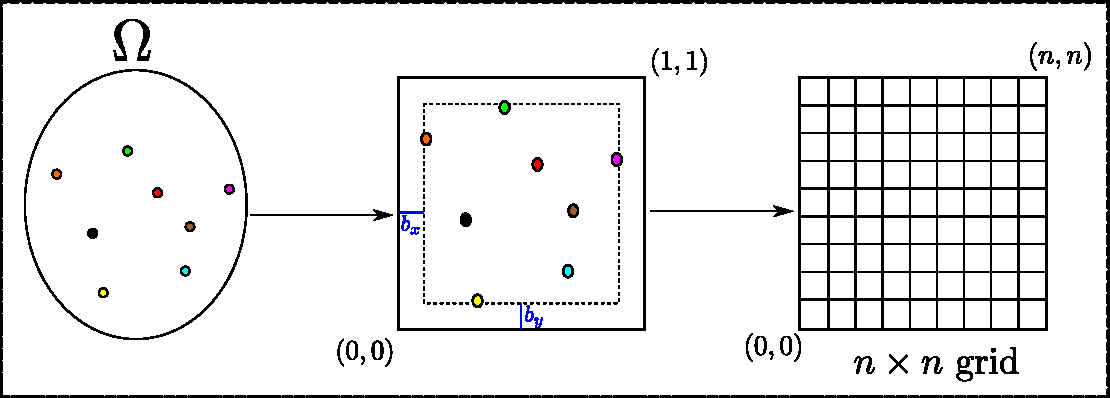
\includegraphics[scale=0.5]{./continuoamalla.pdf}
	\end{center}
	
	First, let $O=(mx,my)$ and $W=(Mx,My)$, where $mx,my,Mx,My$ denote the minimum and maximum points in the dataset. Let $F=W-O$.

	Then, $b_x = R/|F_x|$ and $b_y = R/|F_y|$ are the $x$ and $y$ borders respectively. Any element of the grid outside the border would, by the definition of $R$, contain a number that is less than $\varepsilon$ and therefore can be ignored.
	
	Also, $C$ has to be transformed into $C_x$ and $C_y$ by the equation \tcr{look it up in the code}, because of \tcr{Daniele said so. I agreed he was correct, but I don't remember.}

	\subsection{Finding \texorpdfstring{$w$}{w}}
	
	Once we have $\mu$ for every species, it's time to calculate $\int \mu_A\mu_B$ for every pair of species $\cA$, $\cB$. The straightforward approach has a complexity of $O(s^2n^2)$, where $s$ is the number of species and $n$ is the size of the grid. 
	
	Note the following speedup. Note that 
		$$\int \mu_A \mu_B \approx \sum_{0\leq x < n} \sum_{0\leq y < n} \mu_A[x,y]\mu_B[x,y]$$
	
	If we flatten the matrix $\mu_A$ and $\mu_B$ to vectors $\nu_A$ and $\nu_B$, this last sum is simply the dot product $\nu_A\cdot \nu_B$.
	
	So consider the $s\times n^2$ matrix 
	$$M = \begin{bmatrix}
	        \longleftarrow & \nu_0 & \longrightarrow \\
	        \longleftarrow & \nu_1 & \longrightarrow \\
	        \dots & \dots & \dots \\
					\longleftarrow & \nu_{s-1} & \longrightarrow \\
	      \end{bmatrix}
$$
Then, $MM^T$ is an $s\times s$ matrix whose $(i,j)$-th entry contains $\int \mu_A \mu_B$. This can be done efficiently with fast matrix multiplication algorithms (\cite{strassen}) \tcr{(Marisol, tú te los sabes seguramente, pon unas palabritas de ellos y di que son super chidos y que no se que)}.

Note also that the algorithms described here are highly parallelizable, and indeed the code uses as many cores as available.

\section{Experiments and results}

\subsection{Digraphs}
The following digraphs were obtained as a result of the algorithms described in the previous section. \tcr{(mm... damos las gráficas? La más chica es una matriz de $56\times56$, aunque podríamos dar sólo las aristas más pesadas... no sé)}

\subsection{Analysis of the digraphs}
This graphs are cool because here is the robustness and the analysis revealed deep and important truths \tcr{(Yo les doy los resultados del análisis. Uds. escriben por qué, para qué, cómo, cuándo, etc.)}



\section{Conclusions}

Finally, we conclude this awesome work. Please accept this paper!!


\section*{Acknowledgements}

This project was supported by PAPIIT IA106316.


\bibliographystyle{myamsalpha}
\bibliography{references}

\end{document}